%% Document class
\documentclass[iop,revtex4,numberedappendix,appendixfloats]{emulateapj}

%% General packages
\usepackage{amsmath}
\usepackage{mathrsfs }
\usepackage{lscape}

%% Figure packages
\usepackage{grffile}
\usepackage{subfigure}

%% Referencing
\usepackage{hyperref}

%% Custom macros
\newcommand{\vect}[1]{\boldsymbol{#1}}
\newcommand*\diff{\mathop{}\!\mathrm{d}}
\newcommand*\Diff[1]{\mathop{}\!\mathrm{d^#1}}
\newcommand{\pdf}{\ensuremath{pdf}}
\newcommand{\pmodel}{\ensuremath{p_M}}
\newcommand{\MAP}{MAP}
\newcommand{\MAPs}{MAPs}
\newcommand{\RM}{{\sl RoadMapping}}
\makeatletter
\newcommand{\testlabel}[2]{%
 \protected@write \@auxout {}{\string \newlabel {#1}{{#2}{\thepage}{#2}{#1}{}} }%
 \hypertarget{#1}{#2}
}
\makeatother

\usepackage[usenames,dvipsnames]{xcolor}
\newcommand{\Wilma}[1]{\textcolor{Magenta}{#1}}
\newcommand{\HW}[1]{\textcolor{Green}{#1}}
\newcommand{\Jo}[1]{\textcolor{Blue}{#1}}

%% Abbreviations
\shorttitle{The Influence of Spiral Arms on Action-based Dynamical Modelling of the Milky Way Disk}
\shortauthors{Trick et al.}

\begin{document}

%-----------------------------------------------------------------------------------------------------------------------------------------------------------------------------
%TITLE
%-----------------------------------------------------------------------------------------------------------------------------------------------------------------------------
\title{The Influence of Spiral Arms on Action-based Dynamical Milky Way Disk Modelling\\}

%% Authors
\author{Wilma H. Trick\altaffilmark{1,2}, Jo Bovy\altaffilmark{3}, Elena D'Onghia\HW{???}, and Hans-Walter Rix\altaffilmark{1}}

%% Affiliations
\altaffiltext{1}{Max-Planck-Institut f\"ur Astronomie, K\"onigstuhl 17, D-69117 Heidelberg, Germany}
\altaffiltext{2}{Correspondence should be addressed to trick@mpia.de.}
\altaffiltext{3}{Department of Astronomy and Astrophysics, University of Toronto, 50 St. George Street, Toronto, ON, M5S 3H4, Canada}

%-----------------------------------------------------------------------------------------------------------------------------------------------------------------------------
%ABSTRACT
%-----------------------------------------------------------------------------------------------------------------------------------------------------------------------------

\begin{abstract}
\begin{itemize}
\item One sentence on what RoadMapping is.
\item Overall axisymmetric RoadMapping modelling works in the presence of non-axisymmetric spiral arms, as long as spiral arms do not dominate too much.
\item Our simple assumption for a DF, a single qDF, seems to be surprisingly successful in modelling the snapshot galaxy.
\item Forces can be reliably recovered at the position of the stars that entered the analysis, with only small biases induced by the spiral arms.
\item A survey volume of $r_\text{kpc}=3~\text{kpc}$ gives equally good constraints on a spatially averaged radial and vertical forces as a volume with $r_\text{max}=5~\text{kpc}$. However, only the latter seems to be able to recover the true halo scale length. 
\end{itemize}
\end{abstract}

%-----------------------------------------------------------------------------------------------------------------------------------------------------------------------------
%KEYWORDS
%-----------------------------------------------------------------------------------------------------------------------------------------------------------------------------
\keywords{Galaxy: disk --- Galaxy: fundamental parameters --- Galaxy: kinematics and dynamics --- Galaxy: structure --- \Wilma{[TO DO]}}

%-----------------------------------------------------------------------------------------------------------------------------------------------------------------------------
%INTRODUCTION
%-----------------------------------------------------------------------------------------------------------------------------------------------------------------------------
\section{Introduction}

The first step in learning more about the Milky Way's (MW) overall gravitational potential and orbit distribution function (DF)---which are crucial for understanding galaxy structure and formation---is to find the ``best possible'' axisymmetric model for the Galaxy. Given such a model the identification and characterization of non-axiysmmetries like the bar, spiral arms or stellar streams in stellar phase-space (and chemical abundance) data would then become more straightforward.

Several approaches to constrain an axisymmetric potential and/or orbit DF have recently been put forward: \citet{2013ApJ...779..115B} and \citet{2014MNRAS.445.3133P} fitted potential and DF simultaneously to stellar kinematics in the disk and got precise constraints on the overall potential; \citet{2015MNRAS.449.3479S} and \citet{2016MNRAS.tmp..817D} investigated extended DFs for the disk and halo respectively (given a fiducial potential), that included in addition to the distribution in orbit space also metallicity of the star. 

In this work we will continue our investigation of the \RM{} approach (\emph{``Recovery of the Orbit Action Distribution of Mono-Abundance Populations and Potential INference for our Galaxy''}). The first application of \RM{} was done by \citet{2013ApJ...779..115B} and \citet{Trick 2016}, hereafter Paper I, performed a detailed analysis of the strengths and weaknesses of the approach. 

The idea behind \RM{} is, that simple stellar populations in the MW disk---be it mono-abundance populations \citep{Bovyabcd, ting} \Wilma{TO DO} (i.e., stars with the same $[\mathrm{Fe}/\mathrm{H}]$ and $[\alpha/\mathrm{H}]$ \Wilma{Check}) or maybe also mono-age populations \Wilma{[References: Maybe Martig??? Any Bovy reference about age???]}---follow simple orbit DFs, like, e.g., the quasi-isothermal DF (qDF) by \citet{???}. Given an assumed gravitational potential one can calculate the orbits---or specifically the orbit's actions $\vect{J}=(J_R,J_\phi=L_z,J_z)$, which are integrals of motions---from the star's current phase-space position $(\vect{x},\vect{v})$. Only if the assumed gravitational potential is realistic, this orbital action distribution will follow a realistic orbit DF like the qDF. This allows one to simultaneously fit potential and orbit DF to observations.

\citet{2013ApJ...779..115B} employed this approach to measure the Milky Way's surface density profile within $1.1~\text{kpc}$ using \Wilma{how many?} MAPs in the Galactic disk from the SEGUE survey \Wilma{Check} \Wilma{Reference}. Their potential model had only two \Wilma{Check} free parameters (disk scale length and halo contribution to the radial force at the solar radius). To account for missing model flexibility they constrained the surface density for each MAP only at one best radius. The profile they derived in this fashion had a scale length of $R_s=2.5~\text{kpc}$ and was---in the regime $R>6~\text{kpc}$ \Wilma{Check}---later confirmed by \citet{2014MNRAS.445.3133P} using a different action-based procedure.

Given the success of this first application and in anticipation of the upcoming data releases from Gaia in 2016-2022 \Wilma{Check}, \Wilma{Trick et al. 2016} improved the \RM{} machinery and studied its strengths and breakdowns in detail, by investigating a large suite of mock data sets. Under the prerequisite of axisymmetric data and model, they found that \RM{}'s modelling success is stable against minor misjudgements of DF or selection function, and that---if the true potential is not contained in the proposed family of model potentials---one can still find a good fit, given the limitations of the model. Paper I also found that measurement uncertainties of the order of those by the final Gaia data release should be good enough (within $3~\text{kpc}$ from the Sun) to allow for precise and unbiased modelling results. 

\Wilma{[TO DO: Continue]}

What was not investigated in Paper I, was the breakdown of axisymmetry in the data and what would happen if both axisymmetric distribution function and potential models would therefore not contain the true DF and potential anymore. This will be this work's subject of investigation.

Here we will specifically investigate the important question, if axisymmetric \RM{} modelling can still give reliable constraints on the potential in the presence of non-axisymmetric spiral arms in the data.


\begin{itemize}
\item 
\item Main question: Does axisymmetric RoadMapping modelling work in the presence of non-axiysmmetric spiral arms?
\item Consequences: Both potential and orbit DF are not axisymmetric, i.e., the fitted axisymmetric potential model and DF do per se not contain the truth.
\item How to approach this: Use simulation by D'Onghia et al. 2013 and apply RM to it
\item The potential model we use is chosen mostly for practical reasons and is not necessarily the optimal one for the simulation. Also, we use a single qDF as DF - because it is the simplest thing to do. Also independently of the non-axisymmetries the chosen models might deviate from the truth. Where we investigated deviations between model and truth in isolated test cases, here several assumptions break down simultaneously.
\item Explain actions very shortly. $\vect{J}=(J_R,J_\phi=L_z,J_z)$ quantify oscillation in the coordinate directions $(R,\phi,z)$. Are calculated from current phase-space position in a given potential $\Phi$.
\item Say that actions are conserved in an axisymmetric potential, but not in non-axisymmetric potentials. (Maybe the mean vertical action is conserved \Wilma{[TO DO: Reference]}.) It is therefore important to check, if our modelling works in a system where actions are not conserved.
\end{itemize}

%-----------------------------------------------------------------------------------------------------------------------------------------------------------------------------
%SIMULATION
%-----------------------------------------------------------------------------------------------------------------------------------------------------------------------------
\section{Data from a galaxy simulation} \label{sec:simulation}

%====================
\begin{figure}[!htbp]
\plotone{fig/plot_simulation_for_paper.pdf}
\caption{Simulation snapshot by \citet{2013ApJ...766...34D} . Shown are the surface mass density (in $(x,y)$ plane, upper panel) and mass density (in $(R,z)$ plane, lower panel) of the ``star'' particles belonging to disk, bulge and giant molecular clouds. (The dark matter halo in this simulation is static and analytic and not shown here.) Overplotted are the disk's scale length $R_s=2.5~\text{kpc}$ (see Section \ref{sec:simulation_description}) and the radii at which we center our test survey volumes in this investigation, $R=8$ and $5~\text{kpc}$. The centers of the different survey volumes are marked with a square, if the survey volume is centered on a spiral arm, or with a circle, if the volume is centerd on an inter-arm region. The yellow circle with radius $r_\text{max}=4~\text{kpc}$ marks the survey volume in which we conduct the analysis discussed in detail in Section \ref{sec:results_part1}. \Wilma{[TO DO: Rename $R_{disk}$ to $R_s$ as it is the scale length of the disk.]}}
\label{fig:simulation}
\end{figure}
%====================

\subsection{Description of the galaxy simulation snapshot} \label{sec:simulation_description}

In this work we use stellar phase-space data drawn from high-resolution N-body simulation snapshot of a disk galaxy by \citet{2013ApJ...766...34D} carried out with GADGET-3 code described in \citet{2005MNRAS.361..776S}, in which overdensities with properties similar to giant molecular clouds induced prominent spiral arms---and therefore non-axisymmetric sub-structure---via the swing amplification mechanism. 

For details see \citet{2013ApJ...766...34D}, here we summarize the essential characteristics.

The simulation has a gravitationally evolving stellar disk within a static/rigid analytic dark matter halo.

The analytic halo follows a \citet{1990ApJ...356..359H} profile
\begin{equation}
\rho_\text{dm}(r) = \frac{M_\text{dm}}{2\pi} \frac{a_\text{dm}}{r (r+a_\text{dm})^3} \label{eq:dm_hernquist}
\end{equation}
with total halo mass $M_\text{dm} = 9.5\cdot 10^{11} ~M_\odot$ and scale length $a_\text{dm} = 29~\text{kpc}$ (Elena D'Onghia, private communication). \HW{[There is no way to check that this is indeed the case. What should I do?]} \Jo{[What does "total mass computed at 160 kpc mean? What does concentration c=9 mean for a Hernquist halo? How does that fit together with a=29 kpc?]}

The disk consists of $10^8$ ``disk star'' particles, each having a mass of $\sim370 ~M_\odot$, and 1000 ``giant molecular cloud'' particles with mass $\sim9.5\cdot 10^{5} ~M_\odot$. Initially the particles are distributed following an exponential disk profile with density
\begin{equation*}
\rho_*(R,z) = \frac{M_*}{4\pi z_0 R_s^2} \text{sech}^2 \left( \frac{z}{z_0}\right) \exp \left(- \frac{R}{R_s} \right),
\end{equation*}
with $R_s = 2.5~\text{kpc}$ and $z_0=0.1R_s$ \Wilma{[TO DO: Check in my own measurements]} and total disk mass $M_* = 0.04\cdot M_\text{dm} = 3.8\cdot 10^{10} M_\odot$ .

The bulge consists of $10^7$ ``bulge star'' particles with mass $\sim950 ~M_\odot$ and they are distributed following a spherical Hernquist profile analogous to Equation \eqref{eq:dm_hernquist}, with total mass $M_\text{bulge}=0.01 \cdot M_\text{dm} = 9.5\cdot 10^9~M_\odot$ and scale length $a_\text{bulge}=0.1\cdot R_s=0.25~\text{kpc}$.

The simulation snapshot which we are using in this work has evolved under its own gravity for $\sim 250~\text{Myr}$, which corresponds to approximately one orbital period at $R\sim8~\text{kpc}$. The mass density of simulation particles (without the DM halo) at this snapshot time is shown in Figure \ref{fig:simulation}. Pronounced spiral arms have developed due to the ``molecular cloud perturbers'', which can be seen in Figure \ref{fig:simulation} as small overdensities in the disk. The spherical bulge and very flattened disk are shown in the lower panel in Figure \ref{fig:simulation}.

We have confirmed that the gravitational center of the particles corresponds to the coordinate origin.

\subsection{Survey volume and data}

The selection function of all-sky surveys like Gaia, that are only limited by the brightness of the tracers, are contiguous and---when ignoring anisotropic effects like dust obscuration---spherical in shape. For simplicity we will use spherical survey volumes centered on different vantage points and with sharp edges at a radius $r_\text{max}$ around it (see also Section \ref{sec:likelihood}), which corresponds to a magnitude cut for stellar tracers all having the same luminosity. Figure \ref{fig:simulation} illustrates the different survey volume positions we use in this study: We use each a volume with $r_\text{max}=1,2,3,4$ or $5~\text{kpc}$ centered on a spiral arm and on an inter-arm region at both the equivalent of the solar radius in this simulation, $R=8~\text{kpc}$, and at $R=5~\text{kpc}$, where the spiral arms are more pronounced (see Figure \Wilma{[TO DO: Make plot that illustrates strengt of spiral arm and reference it here]}) than at $R=~\text{kpc}$. From each volume we draw $N_*=20,000$ random ``disk star'' particles from the simulation and use their phase-space positions $(\vect{x}_i,\vect{v}_i)$ within the simulated galaxy's restframe as data. To make the data sample more realistic, one would actually have to add measurement uncertainties, especially to the distances of the survey volumes central vantage point and the proper motions measured from there. We decided not to include measurement uncertainties: Firstly, their effect on \RM{} modelling has been already investigated in Paper I and we found that the measurement uncertainties of the last data release of Gaia should be small enough to not disturb the modelling to much. Secondly, in this study we want to isolate and investigate the deviations of the data from the assumed potential and DF model and axisymmetry independently of other effect.

\Wilma{[TO DO: Add a table that introduces names for the positions S8, S5, I8, I5, and lists their coordinates.]}

\subsection{Symmetrized potential model} \label{sec:DEHH-Pot}

For a galaxy with pronounced spiral arms an axisymmetric model matter distribution can per se not reproduce the true matter distribution globally. We derived an \emph{overall best fit symmetrized} potential model from the distribution of particles to be able (i) to quantify the non-axisymmetries in the simulation snapshot better and (ii) to compare how close our axisymmetric \RM{} results can get to it. 

We derive this model by fitting axisymmetric analytical functions to the density distribution of each of the galaxy component's particles: The bulge and halo follow each a Hernquist profile by construction (see Section \Wilma{[TO DO]}). The disk with its spiral arms however does deviate strongly from its initial conditions in Equation \Wilma{???}. We chose the double exponential disk model from the \texttt{galpy} (galaxy python) library to fit the particle distribution in the disk. (This profile is better than the Miyamoto-Nagai disk in reproducing the overall radial density slope, but as it has not the advantage of allowing fast force calculations, we are not using it in the \RM{} modelling.) The best fit parameters for this reference potential, to which we will refer as the \texttt{DEHH-Potential} (Double-Exponential disk + Hernquist halo + Hernquist bulge) in the remainder in this work, are given in Table \Wilma{[TO DO]}. As can be seen in Figures \Wilma{[TO DO]} in Section \Wilma{[TO DO]} below, the \texttt{DEHH-Pot} fits the overall density distribution very well. Its density profile might be a little stepper around $z~sim0$ than the actual particle distribution, but this should not affect the overall discussion, as the radial density, surface density and disk-to-halo ratio profiles are so well reproduced.

Globally our \RM{} model can not be better than this \emph{overall best fit symmetrized} \texttt{DEHH-Pot}, which acts therefore like a global upper limit to \RM{}. We note that in deriving the \texttt{DEHH-Pot} we used the correct decomposition into bulge, disk and halo components, while \RM{} only feels the composite gravitational effect. Given the flexibility of the potential model \texttt{MNHH-Pot} used in \RM{} and the restriction of the modelling to a survey volume, it could however be possible that \RM{} can do better in fitting the local potential inside the survey volume at the price of recovering the global potential parameters to less accuracy. We will discuss this in the following sections.




%====================
\begin{deluxetable}{lll}[!htbp]
\tabletypesize{\scriptsize}
\tablecaption{Best fit parameters of the \texttt{DEHH-Pot} (see Section \Wilma{[TO DO]}), which we use as the global best fit symmetrized potential model. \label{tbl:DEHH-Pot}}
\tablewidth{0pt}
\startdata
\tableline
circular velocity & $v_\text{circ}(R_\odot)$ & $222~\text{km s}^{-1}$ \\
disk scale length & $h_r$ & $2.5~\text{kpc}$ \\
disk scale height & $h_z$ & $0.17~\text{kpc}$ \\
halo fraction & $f_\text{halo}$ & $0.54$\\
halo scale length & $a_\text{halo}$ & $29~\text{kpc}$ \\
bulge fraction & \Wilma{[TO DO]} & \Wilma{[TO DO]} \\
bulge scale length & \Wilma{[TO DO]} & \Wilma{[TO DO]}
\enddata
%\tablenotetext{(a)}{...}
\end{deluxetable}
%====================

\subsection{Quantifying influence of spiral arm}

\Wilma{[TO DO: There is a short comment on that in D'Onghia 2013 as well]}

\Wilma{[TO DO: Maybe give the different survey centroids names A,B,C,D, so it's easier to talk about them.]}

Depending on size and position of the survey volume the spiral arms and inter-arm regions dominate the stellar distribution within the survey volume to different degrees. To quantify the strength of the spiral arm, we introduce the quantity
\begin{equation*}
\kappa(x_j,y_j) \equiv \frac{\Sigma_{\text{disk},T}(x_j,y_j \mid |z|\leq 1.5~\text{kpc})}{\Sigma_{\text{disk},S}(x_j,y_j \mid |z| \leq1.5~\text{kpc})} -1
\end{equation*}
where $\Sigma_{\text{disk},i}$ is the surface density of the disk component  of the simulation snapshot ($i=T$) or of the symmetrized snapshot model \texttt{DEHH-Pot} in Section \ref{sec:DEHH-Pot} ($i=S$) within the survey volume,
\begin{equation}
\Sigma_{\text{disk},i} \equiv \int_{-1.5~\text{kpc}}^{1.5~\text{kpc}} \rho_{\text{disk},i}(x_j,y_j,z) \ \diff z.
\end{equation}
$(x_j,y_j)$ is the centroid of a surface area element $(x_j\pm\delta,y_j\pm \delta)$ with $\delta=0.25~\text{kpc}$. $(x_c,y_c,z_c=0)$ is the position of the survey volume's center within the simulation's cartesian coordinate system, $c\in\left\{ A,B,C,D\right\}$. We consider all $n \simeq \pi r_\text{max}^2/4\delta^2$ values of $\kappa(x_j,y_j)$ inside a given survey volume and calculate the statistics
\begin{eqnarray*}
\langle \kappa (r \leq r_\text{max} | c) \rangle &\equiv& \frac 1n \sum_j^n \kappa(x_j,y_j)\\
\text{and} \Delta \kappa(r \leq r_\text{max} | c) &\equiv& \text{max}[\kappa(r \leq r_\text{max} | c)] - \text{min}(r \leq r_\text{max} | c)]\\
\text{with} && (x_j-x_c)^2 + (y_j-y_c)^2 \leq r_\text{max}.
\end{eqnarray*}
This gives us information if a spiral arm or an inter-arm region dominates the survey volume ($\langle \kappa \rangle > 0$ for spiral arms, $\langle \kappa \rangle < 0$ for inter-arm regions) and how large the contrast between spiral arms and inter-arm regions is ($\Delta \kappa$).

%====================
\begin{figure*}[!htbp]
\centering
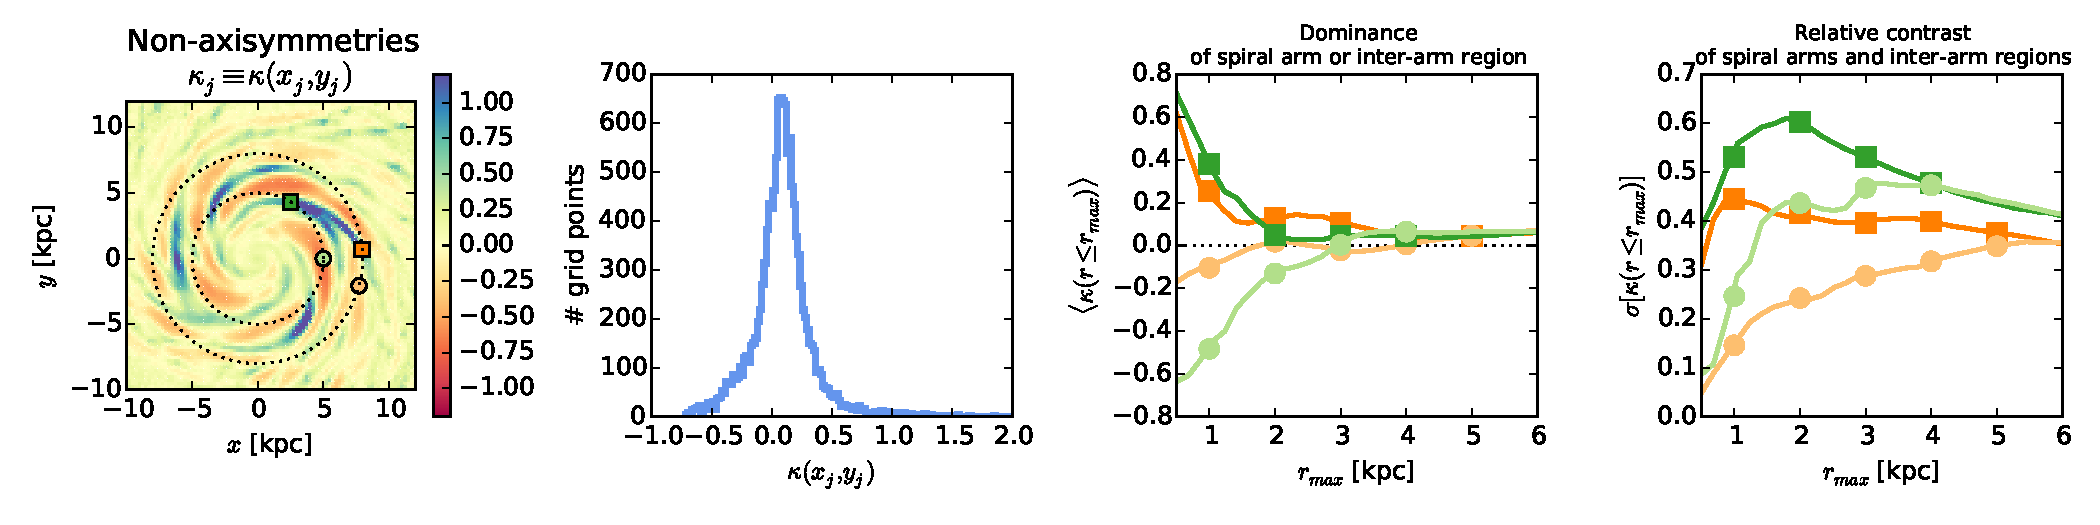
\includegraphics[width=\textwidth]{fig/whole_galaxy_kappa_i.pdf}
\caption{Contrast and dominance of the spiral arms. The left panel shows the values of $\kappa_i$ calculated according to Equation \Wilma{[TO DO]} as described in Section \Wilma{[TO DO]} at regular grid points $(x_i,y_i)$ with bin width $0.25~\text{kpc}$. Marked are the centroids of the four test survey volumes of this study. The second panel shows a histogram over all $kappa(x_j,y_j)$ values in the region $x,y \in [-14,14]~\text{kpc}$. The two right panels show the dominance (with the mean $\langle \kappa (r \leq r_\text{max} \rangle$ of all grid points within the survey volume as measure) and the relative contrast (with the standard deviation $\sigma[kappa (r \leq r_\text{max})]$ as measure) of spiral arms and inter-arm regions inside a spherical survey volume with given centroid (colour-coded) and size (radius $r_\text{max}$ shown on the $x$-axis). We chose two volumes in which the spiral arms dominate, and two in which an inter-arm region dominates. The dominance and contrast of spiral arms and inter-arm regions is stronger at $R=5~\text{kpc}$ than at $R=8~\text{kpc}$. Also, inter-arm regions appear larger and smoother than spiral arms, as already inside a small volume centred on a spiral arm the contrast is quite large. The larger the volume the more does the overall effect of spiral arms and inter-arm regions average out.}
\label{fig:???}
\end{figure*}
%====================


%-----------------------------------------------------------------------------------------------------------------------------------------------------------------------------
%MODELLING
%-----------------------------------------------------------------------------------------------------------------------------------------------------------------------------
\section{RoadMapping modelling}

\subsection{Likelihood} \label{sec:likelihood}

The data that goes into the modelling are the 6D position and velocity coordinates $(\vect{x}_i,\vect{v}_i)$ of $N_*$ stars within the survey volume. For simplicity we use a purely spatial selection function $\text{sf}(\vect{x})$ of spherical shape,
\begin{equation*}
\text{sf}(\vect{x}) \equiv \begin{cases} 1 &\mbox{if } \left| \vect{x}-\vect{x}_0 \right| \leq r_\text{max} \\
0 & \mbox{otherwise} \end{cases},
\end{equation*}
whose maximum radius $r_\text{max}$ defines the boundary of the survey volume and which is centred on $\vect{x}_0 \equiv (R_0,\phi_0,z_0=0)$. Given a parametrized potential model $\Phi(R,z)$ with parameters $p_\Phi$, the $i$-th star is on an orbit characterized by the orbital actions 
\begin{equation*}
\vect{J}_i \equiv \vect{J}[\vect{x}_i,\vect{v}_i \mid p_\Phi].
\end{equation*}
The probability of stars to be on the orbit $\vect{J}_i$ is proportional to a given orbit distribution function $\text{df}(\vect{J})$ with parameters $p_\text{DF}$,
\begin{equation*}
\text{df}(\vect{J}_i \mid p_\text{DF}) \equiv \text{df}(\vect{J}[\vect{x}_i,\vect{v}_i \mid p_\Phi] \mid p_\text{DF}) \equiv \text{df}(\vect{x}_i,\vect{v}_i \mid p_\Phi,p_\text{DF}),
\end{equation*} 
where the latter equivalence arises from the Jacobian determinant between the angle-action coordinates $(\vect{\theta},\vect{J})$ and cartesian phase-space coordinates $(\vect{x},\vect{v})$, which is $\left| \partial (\vect{x},\vect{v}) / \partial(\vect{\theta},\vect{J})\right|=1$ and therefore allows us to treat the $\text{df}$ equivalently as a distribution of current phase-space coordinates or a distribution of orbital actions only, with uniform distribution in the angles $\vect{\theta}$. In some sense, the $\text{df}(\vect{J})$ describes how we expect a realistic stellar population in the MW disk to look like.

The joint likelihood of the $i$-th star being on an orbit $\vect{J}$ in the potential $\Phi$ and being within the survey volume is therefore
\begin{equation*}
\mathscr{L}_i \equiv \mathscr{L}(\vect{x}_i,\vect{v}_i) = \frac{\text{df}(\vect{x}_i,\vect{v}_i\mid p_\phi, p_\text{DF}) \cdot \text{sf}(\vect{x_i})}{\int \text{df}(\vect{x},\vect{v}\mid p_\Phi, p_\text{DF}) \cdot \text{sf}(\vect{x}) \ \Diff3 x \Diff3 v}.
\end{equation*}
The details how we evaluate the likelihood normalisation numerically to sufficiently high enough precision are discussed in Paper I.\footnote{\Wilma{[TO DO: Write what exact numerical accuracy we use and check that it is actually good enough.]}}

In the scenario considered in this paper it can happen that there are a few ($\sim 1$ in 20,000) stars entering the catalogue that are for some reason  on rather extreme orbits, e.g., moving radially directly towards the center. These kinds of orbits do not belong to the set of orbits that we classically expect to make up a overall smooth galactic disk. To avoid that such single stars with very low likelihood mess up the modelling we introduce here a simple outlier model,
\begin{equation*}
\mathscr{L}_i \longrightarrow \max \left( \mathscr{L}_i, \epsilon \cdot \text{median}(\mathscr{L})\right),
\end{equation*}
where $\epsilon = 0.001$ for $N_*=20,000$ stars and $\text{median}(\mathscr{L})$ is the median of all the $N_*$ stellar likelihoods $\mathscr{L}_i$ with the given $p_\Phi$ and $p_\text{DF}$. This outlier model was not used in Paper I.

Following Paper I, we assume for now uninformative flat priors on the model parameters $p_\Phi$ and $p_\text{DF}$ and find the maximum and width of the posterior probability function
\begin{equation*}
pdf(p_\Phi,p_\text{DF} \mid \text{data}) \propto \prod_{i=1}^{N_*} \mathscr{L}_i \cdot prior(p_\Phi,p_\text{DF})
\end{equation*}
using a nested-grid approach and then explore the full shape of the $\pdf$ using a Monte Carlo Markov Chain (MCMC)\footnote{\Wilma{[TO DO: Reference emcee]}}. Full details on this procedure are given in Paper I.

\subsection{DF model} \label{sec:DF_model}

The most simple orbit distribution function exhibiting a disk-like structure may be the quasi-isothermal distribution function (qDF) introduced by \citet{2010MNRAS.401.2318B} and \citet{2011MNRAS.413.1889B}. It  proofed to be a successful model to describe the orbit distribution of individual mono-abundance populations (MAPs) in the Galactic disk \citep{2013ApJ...779..115B,2013MNRAS.434..652T}, that seem to be isothermal in $z$-direction (i.e., ``quasi-isothermal''). Modelling approaches trying to capture the overall disk distribution \citep{2014MNRAS.445.3133P,2015MNRAS.449.3479S} were describing the Galactic disk as a superposition of many qDFs. The qDF, which we already used in Paper I, has the functional form
\begin{eqnarray}
&&\text{qDF}(\vect{J} \mid p_\text{DF}) \nonumber\\
&&= f_{\sigma_R}\left(J_R,L_z \mid p_\text{DF}\right) \times f_{\sigma_z}\left(J_z,L_z \mid p_\text{DF}\right)\label{eq:df_general}\end{eqnarray}
where
\begin{eqnarray}
f_{\sigma_R}\left(J_R,L_z \mid p_\text{DF}\right) &=& n \times \frac{\Omega}{\pi\sigma_R^2(R_g) \kappa}\exp\left(-\frac{\kappa J_R}{\sigma_R^2(R_g)} \right) \nonumber\\
&& \times \left[1+\tanh\left(L_z/L_0\right) \right]\\
f_{\sigma_z}\left(J_z,L_z \mid p_\text{DF} \right) &=& \frac{\nu}{2 \pi \sigma_z^2(R_g)} \exp\left( -\frac{\nu J_z}{\sigma_z^2(R_g)} \right)
\end{eqnarray}
\citep{2011MNRAS.413.1889B}. The guiding-center radius $R_g$, circular frequency $\Omega$, radial/epicycle frequency $\kappa$ and vertical frequency $\nu$ describe the near-circular orbit with given angular momentum $L_z$ in a given potential. Counter-rotating orbits with $L_z < L_0$ are suppressed by the term $\left[1+\tanh\left(L_z/L_0\right) \right]$ (with $L_0 \sim 10~\text{km s}^{-1}~ \text{kpc}$). 
We set the radial stellar tracer density $n(R_g)$ and velocity dispersion profiles $\sigma_z(R_g)$ and $\sigma_R(R_g)$ to
\begin{eqnarray}
n(R_g \mid p_\text{DF}) &\propto& \exp\left(-\frac{R_g}{h_R} \right)\\
\sigma_R(R_g \mid p_\text{DF}) &=& \sigma_{R,0} \times \exp\left(- \frac{R_g-R_\odot}{h_{\sigma,R}} \right)\label{eq:sigmaRRg}\\
\sigma_z(R_g \mid p_\text{DF}) &=& \sigma_{z,0} \times \exp\left(- \frac{R_g-R_\odot}{h_{\sigma,z}} \right)\label{eq:sigmazRg}.
\end{eqnarray}
The free model parameters of the qDF are therefore
\begin{equation*}
p_\text{DF} \equiv \left\{ \ln h_R, \ln \sigma_{R,0}, \ln \sigma_{z,0}, h_{\sigma,R}, h_{\sigma,z}\right\}.
\end{equation*}

Even though we do not have any stellar abundance or age information in the simulation snapshot we are going to investigate (see Section \ref{sec:simulation}) and we therefore cannot define stellar sub-populations for which the assumption of such a simple model might be reasonable, we will still try to model the whole disk with a single qDF---to see how far we can get with the simplest possible model.

\subsection{Potential model} \label{sec:potential_model}

\Wilma{[TO DO]}

\begin{itemize}
\item Introduce MNHH potential model, explain that form of disk was mostly chosen to the closed form expression of $Phi$ which allows for fast calculation. 
\item Mention action calculation and that we tested explicitely that fixing Delta=0.45 and using staeckel interpolation grid does not degrade the analysis
\item \Wilma{Mention and reference galpy.}
\end{itemize}

%-----------------------------------------------------------------------------------------------------------------------------------------------------------------------------
%RESULTS
%-----------------------------------------------------------------------------------------------------------------------------------------------------------------------------
\section{Results}

We run the \RM{} modelling on several data sets drawn from different survey volumes in the simulation snapshot introduced in Section \ref{sec:simulation_description}. In Section \ref{sec:results_part1} we will analyze one of these \RM{} analyses in detail, and in Section \ref{sec:results_part2} we compare the different results for the different data sets.

\subsection{A single application of \RM{}} \label{sec:results_part1}

In this section we will discuss the results of the \RM{} analysis of a single data set. This fiducial data set has $N_*=20,000$ stars that were drawn from the spherical volume with $r_\text{max}=4~\text{kpc}$ centered on a spiral arm at the ``solar'' radius $R=8~\text{kpc}$ shown as yellow sphere in Figure \ref{fig:simulation} (position \texttt{S8}). We use \RM{} to fit a single qDF (see Section \ref{sec:DF_model}) and the potential model \texttt{MNHH-Pot} consisting of a Miyamoto-Nagai disk, a Hernquist halo and a (fixed) Hernquist bulge introduced in Section \ref{sec:potential_model} to it. The best fit parameters are summarized in Table \Wilma{[TO DO]}.

\Wilma{[TO DO: Add a table here that summarizes the best fit parameters for the 4kpc8Spiral analysis.]}

\subsubsection{Recovering the stellar distribution} \label{sec:4kpc8Spiral_DF}

In Figure \ref{fig:4kpc8Spiral_DF_comparison} we compare the configuration phase-space distribution of the 20,000 stars that entered the \RM{} analysis as data with the best-fit stellar distribution, which is given by the action-based qDF and potential model found with \RM{}. We note that the spiral arms introduce very strong non-axisymmetries in the data, both in the spatial and the velocity distribution (especially in $v_R$, where a lot more stars move outside than inside as compared to an axisymmetric model). We therefore compare in Figure \ref{fig:4kpc8Spiral_DF_comparison} the data and fit separately for different spatial regions, $R>$ and $<8~\text{kpc}$ and $\phi<$ and $>5^\circ$. In the region where the spiral arm dominates (blue) the best fit \RM{} model is actually a very poor model. However, what the model underestimates in the spiral arm, it slightly overestimates in the other regions and is therefore indeed something like a good average model for the overall distribution. Especially the region at $R>8~\text{kpc}$ and $\phi<5^\circ$, where neither the spiral arm nor the inter-arm regions dominate strongly, is very well described by the model. This is remarkable because we had no indication beforehand that a single qDF might be at all a good enough model to describe the overall stellar distribution in the simulation snapshot. But it obviously does---apart from the spiral arm of course, which we had no chance to capture anyway.

%====================
\begin{figure*}[!htbp]
  \centering
  \subfigure[DF density residuals.\label{fig:DF_densres}]{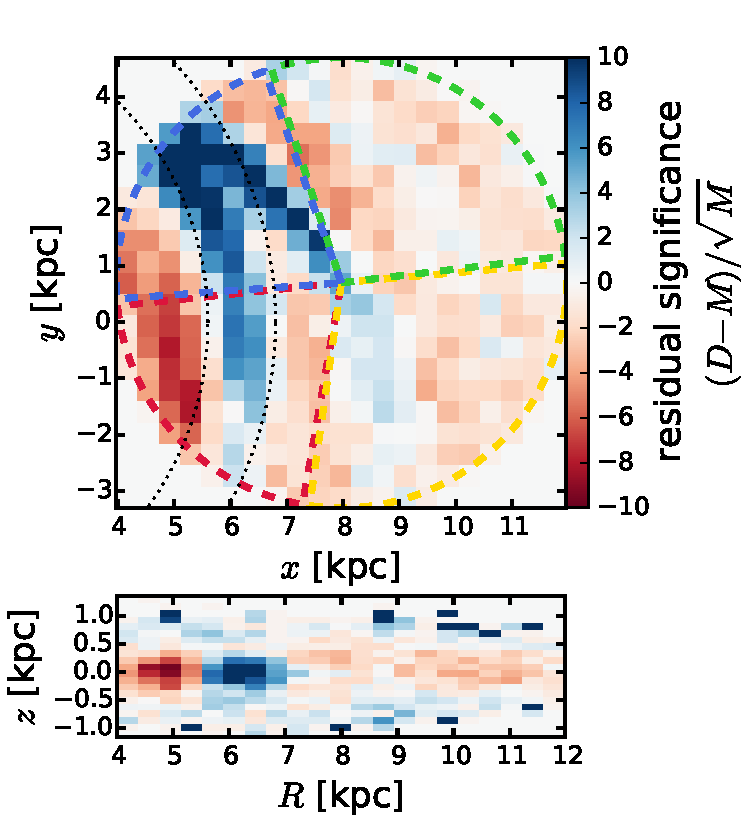
\includegraphics[width=0.32\linewidth]{fig/MNdHHdiffSph2_4kpc8Spiral_a_test1_data_bestfit_residuals_3a.pdf}}
  \subfigure[DF density profiles.\label{fig:DF_densprof}]{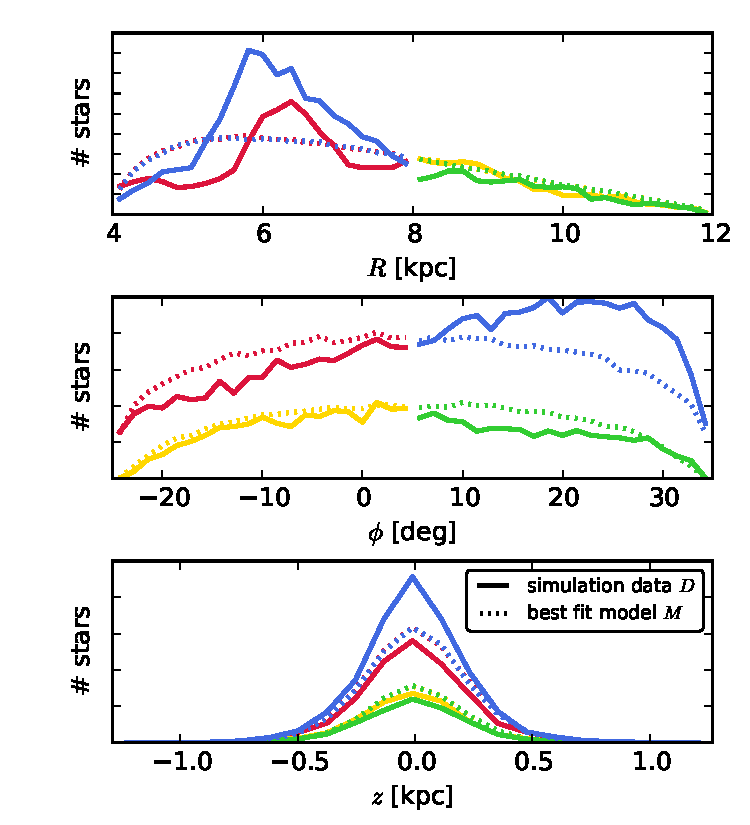
\includegraphics[width=0.32\linewidth]{fig/MNdHHdiffSph2_4kpc8Spiral_a_test1_data_bestfit_residuals_3b.pdf}}
  \subfigure[DF velocity residuals.\label{fig:DF_velres}]{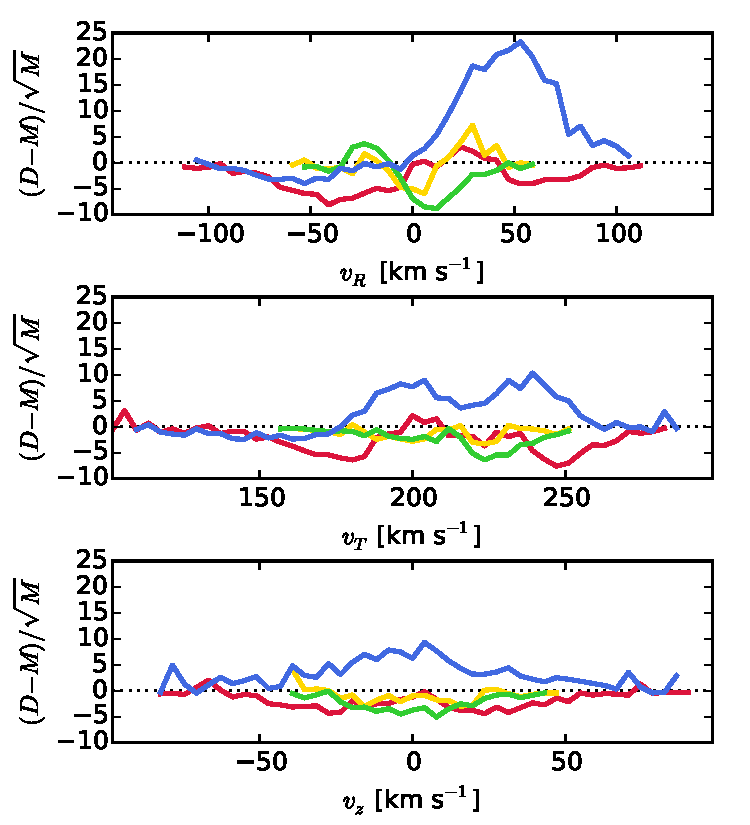
\includegraphics[width=0.32\linewidth]{fig/MNdHHdiffSph2_4kpc8Spiral_a_test1_data_bestfit_residuals_3c.pdf}}
  \caption{Comparison of the DF of stars in position-velocity space in the data set from the simulation snapshot (with $N_*=20,000$ and $r_\text{max}=4~\text{kpc}$ centered on position \texttt{S8}) and in the single-qDF best fit \RM{} model from Table \Wilma{[TO DO]}. Panel \ref{fig:DF_densres} shows the spatial density residual significance projected to the $(x,y)$ and $(R,z)$ plane. In the $(x,y)$ panel the following regions are marked: $R<8~\text{kpc},\phi>5^\circ$ (blue), $R<8~\text{kpc},\phi<5^\circ$ (red), $R>8~\text{kpc},\phi>5^\circ$ (green), $R>8~\text{kpc},\phi<5^\circ$ (yellow). Panels \ref{fig:DF_densprof} and \ref{fig:DF_velres} show the density profiles and velocity residual significance along each of the 6D phase-space coordinates separately for each of the four spatial regions. The blue region is very much dominated by the non-axisymmetric spiral arm. For the yellow region the axisymmetric single-qDF model is a good description. Overall the qDF is a good average axisymmetric model for the data. (In panel \ref{fig:DF_densres} we overplot the radii $R_\text{spiral} \in [5.6,6.8]~\text{kpc}$ as black dotted lines to mark the approximate extent of the stronger spiral arm, to compare it with Figure \ref{fig:4kpc8Spiral_actions}.) \Wilma{[TO DO: Move legend to R panel and make it bigger]}}
  \label{fig:4kpc8Spiral_DF_comparison}
\end{figure*}
%====================


\subsubsection{Recovering the potential} \label{sec:4kpc8Spiral_potential}

As shown in the previous section the best fit \RM{} model seems to reproduce the stellar phase-space distribution quite well. But is the corresponding potential close to the true potential? 

Figures \ref{fig:4kpc8Spiral_density} and \ref{fig:4kpc8Spiral_vcirc_surfdens} compare the true simulation snapshot potential and the axisymmetric \texttt{DEHH-Pot} from Table \ref{tbl:DEHH-Pot} with the best fit \texttt{MNHH-Pot} from the \RM{} analysis. In particular, Figure \ref{fig:4kpc8Spiral_density} illustrates the overall matter density distribution, Figure \ref{fig:4kpc8Spiral_vcirc_surfdens} the rotation curve, surface density profile and disk-to-halo ratio and Figure \ref{fig:4kpc8Spiral_forces} compares the true and recovered (median) gravitational forces at the position of each star in the data set. In Figure \ref{fig:4kpc8Spiral_vcirc_surfdens} we explicitely show the true simulation snapshot circular velocity both averaged over the whole $\Delta\phi=2\pi$ (black lines), and over the survey volume's maximum radial extent $\phi_0\pm \arcsin(r_\text{max}/R_0)$ (grey lines).

The recovery of density, surface density, circular velocity curve and disk-to-halo ratio is especially good in the region where most of the stars are located, around $R\sim~6\text{kpc}$ and in the plane of the disk. In large regions inside the survey volume, and even outside, the density is recovered to within 15\%. The circular velocity curve is even recovered to within 5\%, which is also approximately the extent of perturbation that the spiral arms cause with respect to a smooth rotation curve.

There is however a very small ($<1.5\%$) underestimation of $v_\text{circ}$ at larger radii. We suspect that this is a combination of a bias introduced by the spiral arms (see also discussion in Section \Wilma{[TO DO]}) and the choice of potential model (as a similar bias shows up in the \texttt{DEHH-Pot}). The overall surface density profile is a bit overestimated ($\sim 15\%$) at smaller radii; the reason is clearly the local spiral arm at $R\sim6~\text{kpc}$ with its higher surface density  and many stars entering the analysis, which bias the result and which was to be expected. At larger radii ($R\sim10-12~\text{kpc}$) the fit of radial local density and surface density profile is less good, which we account to the Miyamoto-Nagai disk having a shallower radial profile than an exponential disk, and not enough stars in this outer regions to give good constraints. The much stronger bias in the disk-to-halo ratio at larger radii is the result of a misjudgement of the halo scale length. As we will see later (see Figure \ref{fig:model_parameters}) we seem to need an even larger survey volume to have enough radial coverage to constrain the halo scale length properly. But again, where most of the stars are located, our \RM{} model is a very good average model for the true galaxy.

In Figure \ref{fig:4kpc8Spiral_forces} we compare the true force that each star in the data set feels ($F_{R,T}(*_i)$ and $F_{T,M}(*_i)$, calculated as sum of the individual contributions by each particle in the simulation and the analytic dark matter halo) with the force that the \RM{} median model predicts for each star ($F_{R,M}(*_i)$ and $F_{z,M}(*_i)$). We scale the difference between truth and model by a typical radial or vertical force at the given radius for which we use
\begin{eqnarray}
F_{R,\text{typ}}(R) &\equiv& v^2_{\text{circ},S}(R) / R\\
F_{z,\text{typ}}(R) &\equiv& F_{z,S}(R,z=h_r),
\end{eqnarray}
where $v_{\text{circ},S}$ and $F_{z,S}$ are the circular velocity and vertical force evaluated in the ''true symmetric'' \texttt{DEHH-Pot} in Table \ref{tbl:DEHH-Pot}. As typical vertical force at a given radius we use the vertical force evaluated at the scale height $h_z=0.17~\text{kpc}$ of the disk, because we found that 
\begin{eqnarray*} 
&&\langle |F_{z,S} (*_i)| (R) \rangle \\
&\lesssim& \langle |F_{z,T}(*_i)|  (R) \rangle\\
&\lesssim& F_{z,S}(R,z=h_z) \\
&\lesssim& \langle J_z(*_i) \times \Omega_z(*_i) / h_r \rangle (R),
\end{eqnarray*}
where, e.g., $\langle |F_{z,T}(*_i)|  (R) \rangle$ denotes the mean of the absolute value of the true vertical force of all stars at radius $R$, and $J_z \times \Omega_z \sim \langle E_z \rangle$ is something like the mean vertical energy of a stellar orbit. Figure \ref{fig:4kpc8Spiral_forces} shows therefore
\begin{eqnarray*}
\Delta F_R(*_i) \equiv \left(|F_{R,M}| - |F_{R,T}| \right) / F_{R,\text{typ}}\\
\Delta F_z(*_i) \equiv \left(|F_{z,M}| - |F_{z,T}| \right) / F_{z,\text{typ}}\\
\end{eqnarray*}
for each star. The recovery is as expected: The true vertical force is stronger in the spiral arms (due to the higher surface density) and weaker in the inter-arm regions as compared to the axisymmetric best fit model; the true radial force (i.e., the pull towards the galactic center) is stronger at the outer edge/leading side of the spiral arm because of the additional pull towards the massive spiral arm (and the other way round for the inner edge/trailing side).

%====================
\begin{figure}[!htbp]
\centering
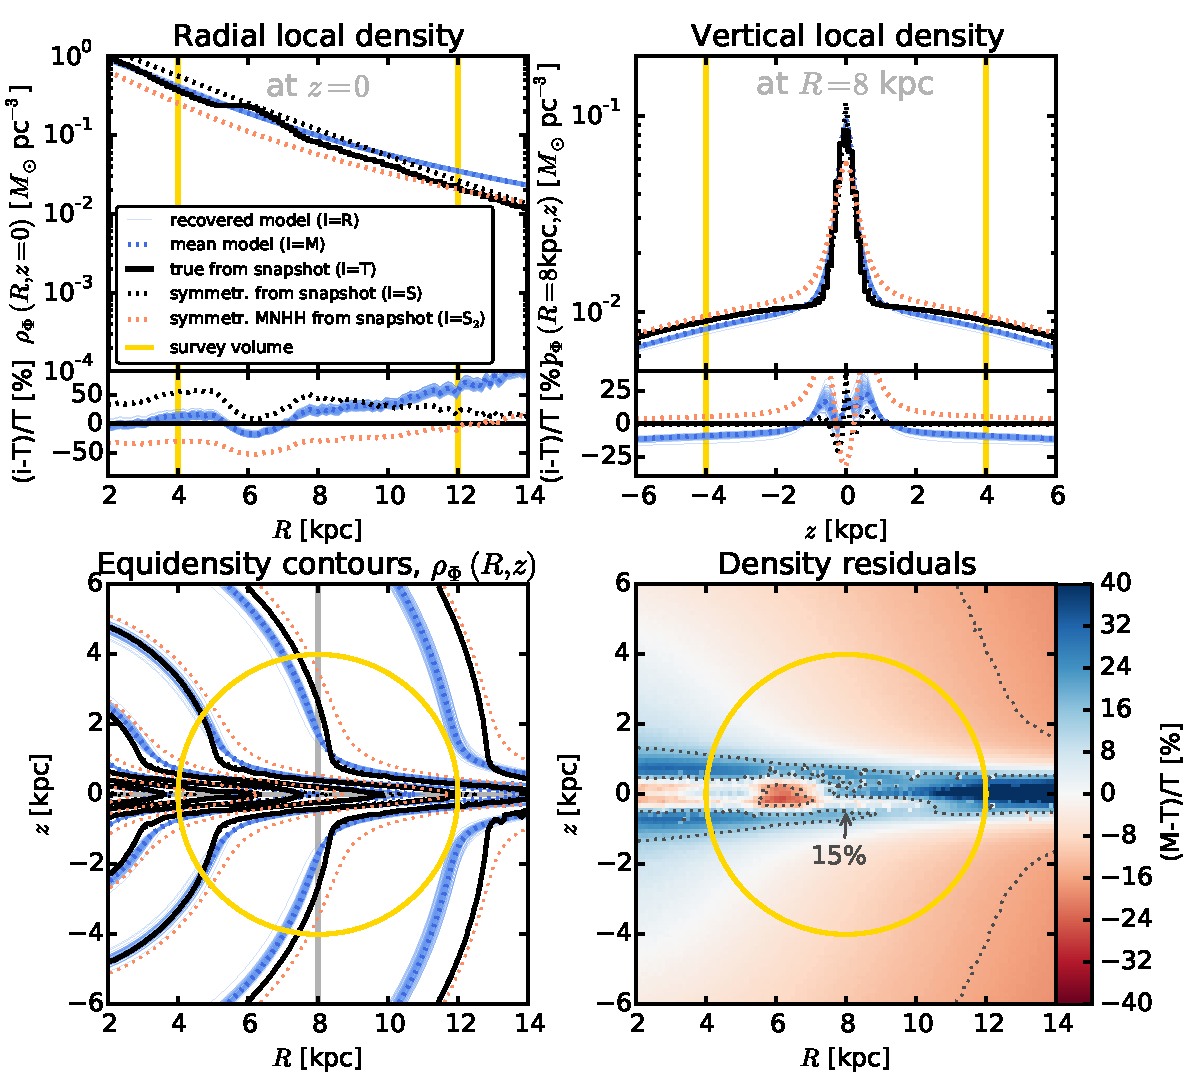
\includegraphics[width=\columnwidth]{fig/MNdHHdiffSph2_4kpc8Spiral_a_test1_density_overview.pdf}
\caption{Comparison of the true density distribution $\rho_{\Phi,\text{T}}$ in the galaxy simulation snapshot (solid black line, averaged over $\phi$) with the axisymmetric density distribution $\rho_{\Phi,\text{R}}$ recovered with \RM{} (solid blue lines) from $N_*=20,000$ stars in the survey volume with $r_\text{max}=4~\text{kpc}$ (yellow line), as described in Section \Wilma{[TO DO]}. The first two panels show density profiles along $(R,z=0)$ and $(R=8~\text{kpc},z)$, together with the relative differences between true and recovered $\rho_{\Phi}$. The third panel displays equidensity contours of the matter distribution in the $(R,z)$ plane. Overplotted are also the overall axisymmetric \texttt{DEHH-Pot}'s $\rho_{\Phi,\text{S}}$ (dotted black line) (see Section \ref{sec:DEHH-Pot}) and the $\rho_{\Phi,\text{M}}$ of the recovered mean model in Table \Wilma{[TO DO]} (dotted blue line). The last panel shows the relative difference between the true $\rho_{\Phi,\text{T}}$ (averaged over all $\phi$) and the recovered mean model $\rho_{\Phi,\text{M}}$. Over wide areas even outside of the survey volume the relative difference is less than $15\%$. At $R\gtrsim8~\text{kpc}$ and $z\sim0$ it becomes apparent that the chosen potential model cannot perfectly capture the structure of the disk. \Wilma{[TO DO: Maybe show the profiles not at R=8 and z=0, but at R=6 and z=$h_z$ or so.]} \Wilma{TO DO: Redo plot. Now I use the median of MCMC samples as best fit model.]}}
\label{fig:4kpc8Spiral_density}
\end{figure}
%====================

%====================
\begin{figure*}[!htbp]
\centering
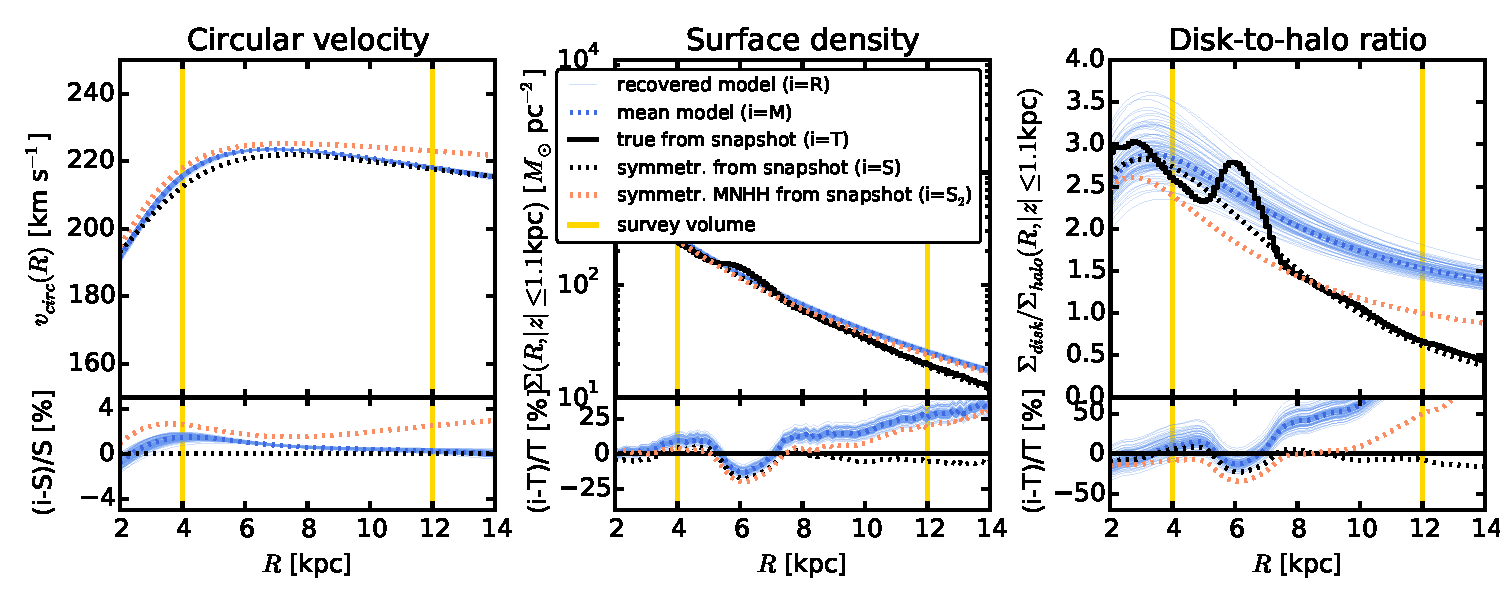
\includegraphics[width=0.7\textwidth]{fig/MNdHHdiffSph2_4kpc8Spiral_a_test1_vcirc_surfdens_overview.pdf}
\caption{\Wilma{[TO DO: Remove MNHH symmetric potential from caption.]} Comparison of the circular velocity curve, surface density profile within $|z|\leq1.1~\text{kpc}$ and disk-to-halo ratio of the surface density along $R$ for the true potential of the galaxy simulation snapshot (solid black line) and the axisymmetric model potential recovered with \RM{} (solid blue lines) (see Section \Wilma{[TO DO]}). Overplotted are also the profiles of the symmetrized ''true´´ potential (dotted black line) (see Section \Wilma{[TO DO]} and Table \ref{tbl:DEHH-Pot}) and the recovered mean model (dotted blue line) (see Table \Wilma{[TO DO]}). The circular velocity curve is recovered to less than $5\%$, especially at larger radii. For the surface density and disk-to-halo ratio \RM{} recovers the truth at radii $\lesssim 8~\text{kpc}$. The deviations at larger radii are connected to the discrepancies in the density in Figure \Wilma{[TO DO]}. \Wilma{[TO DO: Add grey curve for disk to halo ratio.]}}
\label{fig:4kpc8Spiral_vcirc_surfdens}
\end{figure*}
%====================

%====================
\begin{figure}[!htbp]
\centering
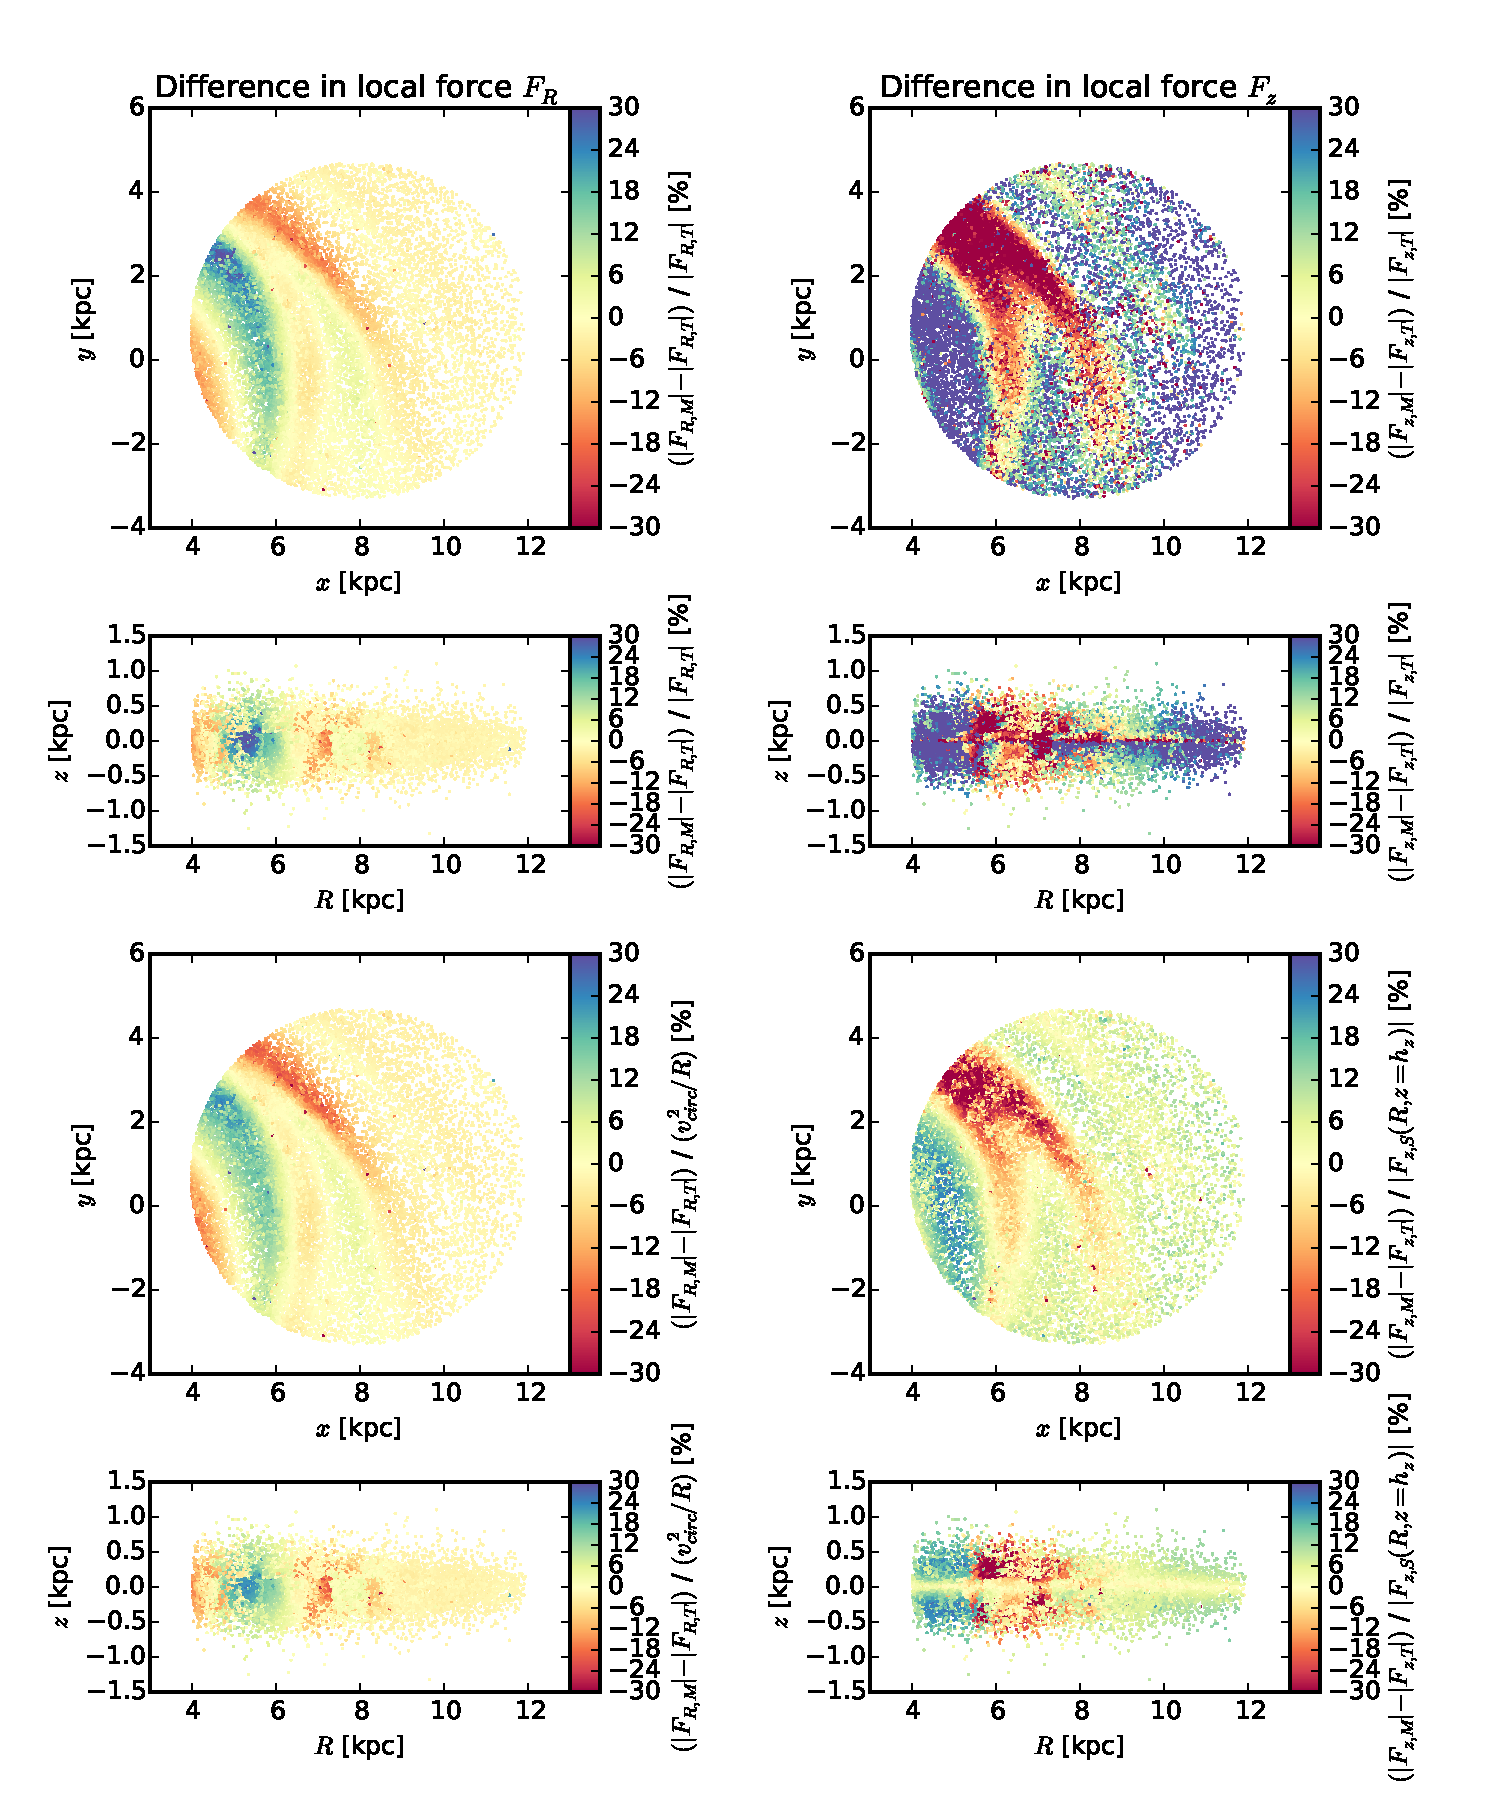
\includegraphics[width=\columnwidth]{fig/MNdHHdiffSph2_4kpc8Spiral_a_test1_forces_overview_5.pdf}
\caption{\Wilma{[TO DO: Rewrite. Figure was replaced.]} Comparison of radial and vertical forces  $F_R=-\partial \Phi / \partial R$ and $F_z = -\partial \Phi / \partial z$ of the true (upper two rows) or symmetrized (lower three rows, black and orange dotted lines) potential of the galaxy simulation snapshot with the potential model recovered with \RM{} (solid blue lines in lower three rows). The upper two rows show the relative difference between the true potential force at the position of each star that entered the \RM{} analysis, and the recovered potential force. The lower three rows compare contours of equal force and force profiles along lines of constant $R$ and $z$. Overall the radial forces are very well recovered, which is related to the well recovery of the circular velocity curve in Figure \Wilma{???}. There are more problems with the vertical force, which is related to the higher surface densities in spiral arms and lower surface density in inter-arm regions, for which the axisymmetric model can only give a average solution. Also, the potential model is not the optimal model to describe the vertical density profile, which becomes also visible in the recovery of the vertical force close to the plane of the disk. \Wilma{[TO DO: Might be, that I have to re-calculate the forces for some of the stars. Write Test that tests if force >1e10 and then recalculates those forces.]} \Wilma{[TO DO: Show only the lower panels.]} \Wilma{TO DO: Redo plot. Now I use the median of MCMC samples as best fit model.]}}
\label{fig:4kpc8Spiral_forces}
\end{figure}
%====================


\begin{itemize}
\item As can be seen in Figure \ref{fig:4kpc8Spiral_forces} the model is a good average model for the majority of stars, i.e. in the wide inter-arm regions and also the stars the peaks of the spiral arms. For the wings of the spiral arms the model is less good: in the leading side of the spiral arm the $|F_{R,M}|$ is underestimated because it does not account for the additional pull of the spiral arm, while in the trailing side of the spiral arm $|F_{R,M}|$ is overestimated, as it does not feel the pull away from the Galactic center by the spiral arm.
\end{itemize}

\subsubsection{Recovering the action distribution}

In Sections \ref{sec:4kpc8Spiral_DF} and \ref{sec:4kpc8Spiral_potential} we have demonstrated the goodness of fit in the configuration space of the data, and of the recovered gravitational potential. What \RM{} is actually fitting is however the distribution in action space. Figure \ref{fig:4kpc8Spiral_actions} compares the data and the model action distribution given the best fit \text{MNHH-Pot} in Table \Wilma{[TO DO]}. (We only use this axisymmetric potential to estimate the actions as they enter the fit, and do not calculate the true actions in the true potential.)

We note that the radial and vertical action distribution fits indeed quite well; the axisymmetric model however contains much more stars on close to circular orbits $(J_R \sim 0,J_z \sim 0)$ than the simulation does. In the data set there is an excess of stars in the galactic plane $(J_z\sim0)$ that have more eccentric orbits  than the axisymmetric model would have. In Figure \ref{fig:DF_densres} we have marked the radial extent of the stronger spiral arm with dotted lines ($R_\text{spiral} \in [5.6,6.8]~\text{kpc}$), and over-plotted the corresponding angular momenta $L_z = R_\text{spiral} \times v_\text{circ}(R_\text{spiral})$ in Figure \ref{fig:4kpc8Spiral_actions} as a rough estimate where in action space we expect the stars of this spiral arm. It is again obvious that this spiral arm contains (i) more stars in general and (ii) more stars with eccentric orbits  $(J_R>0)$ which are (iii) located mostly close to the plane $(J_z\sim0)$, as compared to the axisymmetric model. All of this confirms our expectations for orbits in a spiral arm. 


\begin{figure}[!htbp]
\centering
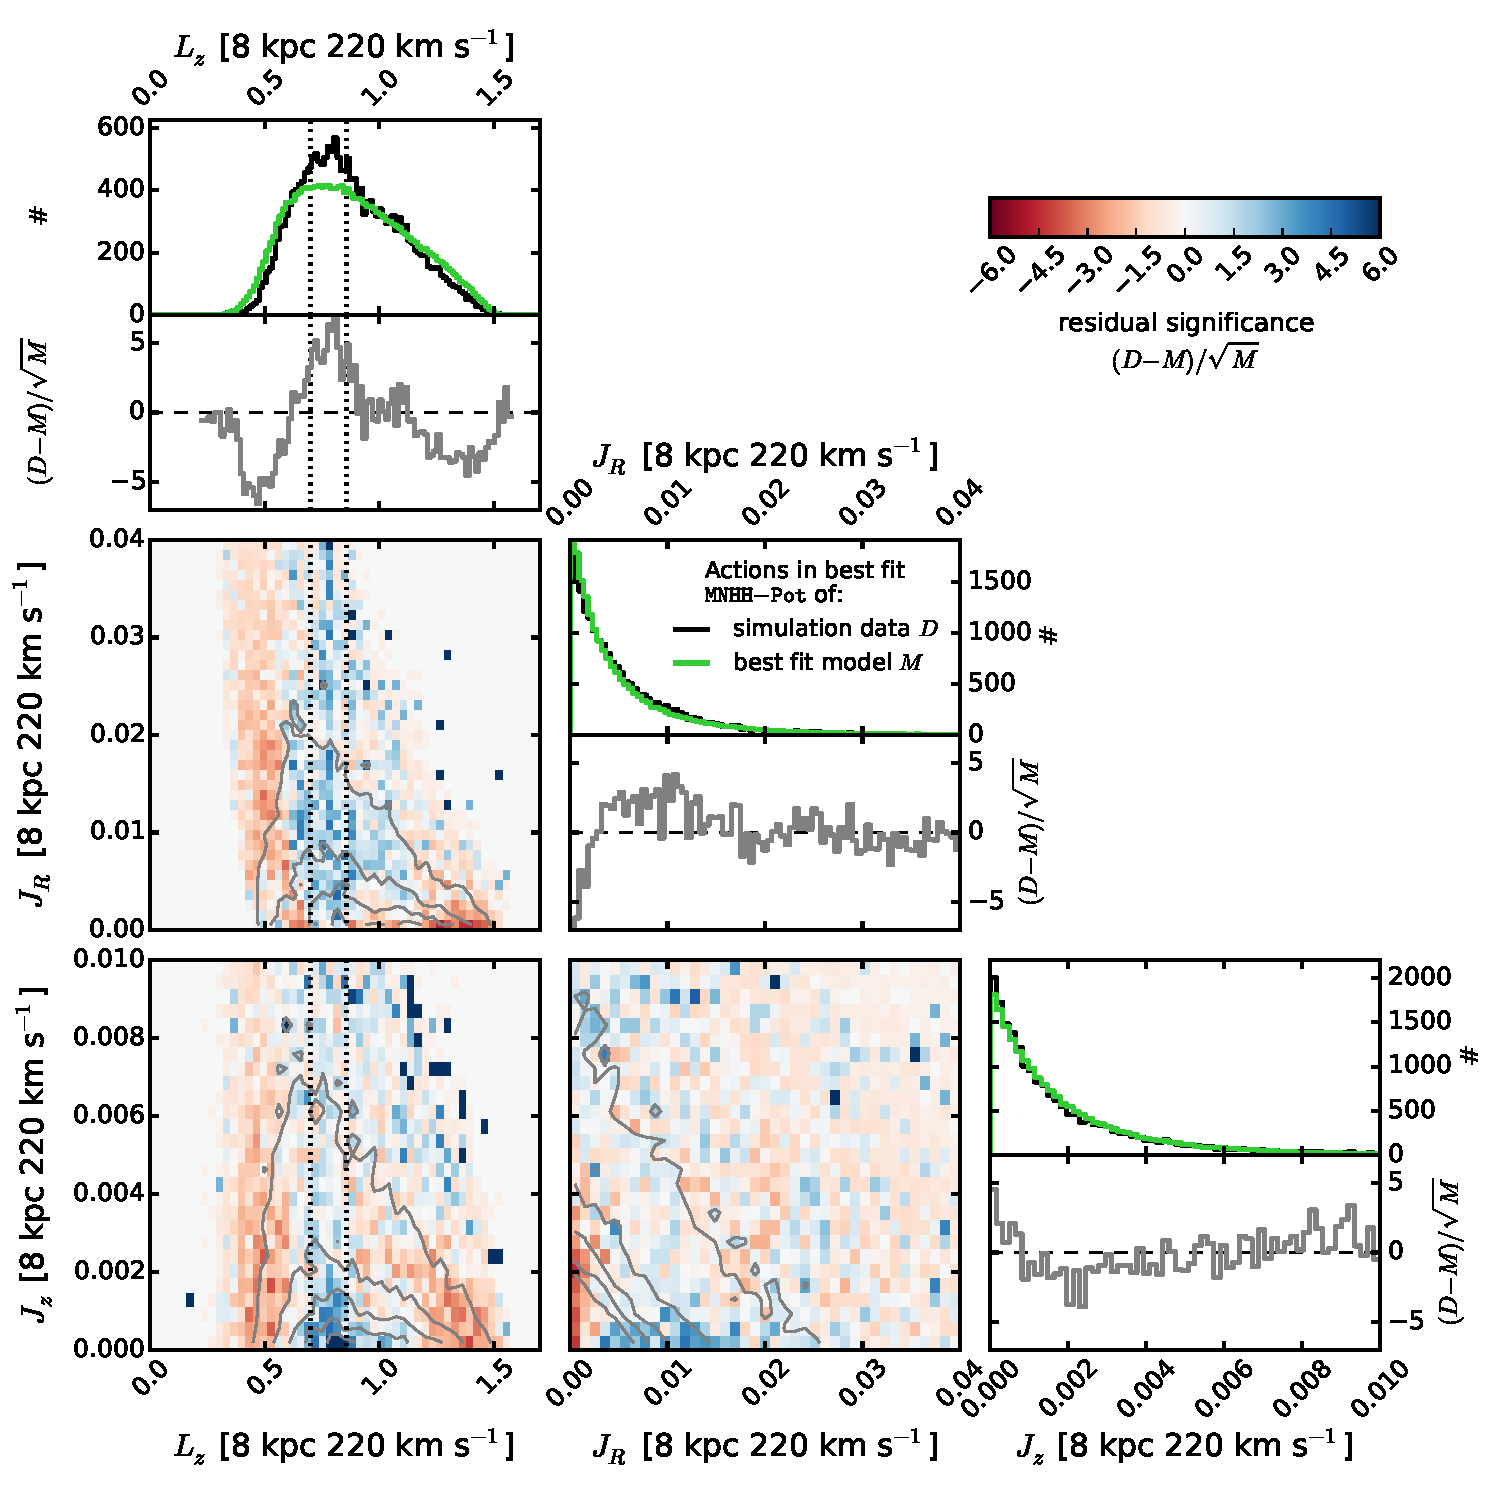
\includegraphics[width=\columnwidth]{fig/MNdHHdiffSph2_4kpc8Spiral_a_data_bestfit_residuals_only_actions.pdf}
\caption{Comparison of the stellar action distribution of the data set $D$ used in the analysis and the recovered axisymmetric stellar distribution $M$ (see Figure \ref{fig:4kpc8Spiral_DF_comparison} for the distribution in configuration space). All actions, of data set and best fit distribution, where calculated in the best fit \texttt{MNHH-Pot} in Table \Wilma{[TO DO]}. The upper panel in each column compares the 1D histograms of the  angular momentum $L_z$, the radial action $J_R$ and the vertical action $J_z$ of both data and best fit. The other 1D and 2D distributions show the residual significance $(D-M)/\sqrt{M}$. The 2D residuals are over-plotted with equidensity contours of the data $D$'s 2D action distribution. In Figure \ref{fig:DF_densres} we have marked the approximate radial extent of the stronger spiral arm with black dotted lines ($R_\text{spiral} \in [5.6,6.8]~\text{kpc}$); the dotted lines in the $L_z$ distributions in this figure correspond to $L_z = R_\text{spiral} \times v_\text{circ}(R_\text{spiral})$.  \Wilma{[TO DO: Ergaenze overall take home message fuer diesen plot.]} \Wilma{[TO DO: Calculate reference data new. Now I use the median of MCMC samples as best fit model.]} \Wilma{TO DO: Redo plot. Now I use the median of MCMC samples as best fit model.]} \Wilma{[TO DO: Add in legend that simulation data was calculated in best fit potential too.]} \Wilma{[TO DO: use the best fit and not the sym model to overplot the dotted lines]}}
\label{fig:4kpc8Spiral_actions}
\end{figure}

\begin{itemize}
\item Figure: residuals in action space, comparison of true/symmetrized vs. best fit actions (maybe also true vs. best fit in symmetrized potential), overplot Lz=vcirc*Rg of spiral arms
\end{itemize}

\clearpage
\newpage

\subsection{The influence of spiral arms on \RM{}} \label{sec:results_part2}

In the previous section we showed that for a large enough survey volume ($r_\text{max}=4~\text{kpc}$) the \RM{} modelling result was a good fit to the data and gave constraints on the gravitational potential which were very close to the true potential. In the following we want to investigate how this modelling success depends on the position and the size of the survey volume.

\subsubsection{Test suite and parameter recovery}

We center our test survey volumes at the positions marked in Figures \Wilma{[TO DO]} and consider volume sizes with $r_\text{max} \in [0,1,2,3,4,5]~\text{kpc}$ for $R_0 = 8~\text{kpc}$ and $r_\text{max} \in [0,1,2,3,4]~\text{kpc}$ for $R_0 = 5~\text{kpc}$. As demonstrated in Figure \Wilma{[TO DO]} the spiral arm strength is very different in these four different test volumes. Each data set contains then $N_*=20,000$ stars inside this spherical volume and we fit a single qDF and \texttt{MNHH-Pot} to it. Figure \ref{fig:model_parameters} shows the best fit parameters for the different \RM{} analyses. We also overplot the parameter of the reference \texttt{DEHH-Pot} in Table \ref{tbl:DEHH-Pot}. Overall the statistical random errors on the parameter recovery are very small for $N*=20,000$ and possible systematic errors dominate. 

Let's first consider the parameters of the gravitational potential: All volumes recover $v_\text{circ}(R_\odot)$ within a few $\text{km s}^{-1}$; in the largest volumes, where the circular velocity curve is probed over several $\text{kpc}$ the estimate is the most accurate. The halo fraction $f_\text{halo}$ of the radial force at the Sun is very well recovered, independent of the size of the volume. The estimate that we get for the best fit Miyamoto-Nagai disk scale height $b_\text{disk}$ seems to be approximately independent of the size of the volume as well. We can even recover the true halo scale length $a_\text{disk}$, however only for a volume as large as $r_\text{max}=5\text{kpc}$. Smaller volumes that underestimate $a_\text{halo}$ get slightly larger estimates for the disk scale length $a_\text{disk}$ and the overall radial density slope is then probably closer to the truth, even if the individual parameters are not.

The right column of Figure \ref{fig:model_parameters} compares the recovered qDF parameters for the different survey volumes with the qDF parameters we got from fixing the potential model to the \text{expHH-Pot} and fitting the qDF only in a $r_\text{max}=5~\text{kpc}$ volume. Even though the qDF parameters for small volumes are widely different for different positions within the galaxy, they all approach the values recovered with the \text{expHH-Pot} for larger volumes. There seems therefore to be indeed an overall best-fit qDF describing the average tracer distribution in the galaxy's disk. The only difference is in the $h_{\sigma,z}$ parameter, where the models with free \texttt{MNHH-Pot} recover a slightly larger value than the models using the known \texttt{expHH-Pot}. The reason is that the Miyamoto-Nagai disk has a different radial profile than the double exponential-disk (see Figure \ref{fig:4kpc8Spiral_density}), which leads to a less steep radial decline in the vertical forces and therefore mean vertical orbital energies $\langle E_z \rangle \sim \nu \times J_z$ and therefore to a slightly longer $h_{\sigma,z}$ scale length. In general, volumes centered on spiral arms have larger velocity dispersion parameters $\sigma_{R,0}$ and $\sigma_{z,0}$ as compared to volumes at the same radius $R$ but centered on an inter-arm region, and the volumes at $R=5~\text{kpc}$ with their stronger spiral arms have larger velocity dispersions than those at $R=8~\text{kpc}$---which is what we expect. Most volumes recover similar tracer scale lengths $h_R$ \Wilma{[TO DO: Value]}; only the volume centered on the inter-arm region at $R=8~\text{kpc}$ recovers much longer $h_R$. This might be related to the fact, that most volumes have strong spiral arms at smaller radii, which leads to estimates of shorter tracer scale lengths, while volume \Wilma{[TO DO: Give different volumes different names. Use 8Void volume here.]} is located in a comparably smooth region of the galaxy.


%====================
\begin{figure}[!htbp]
\centering
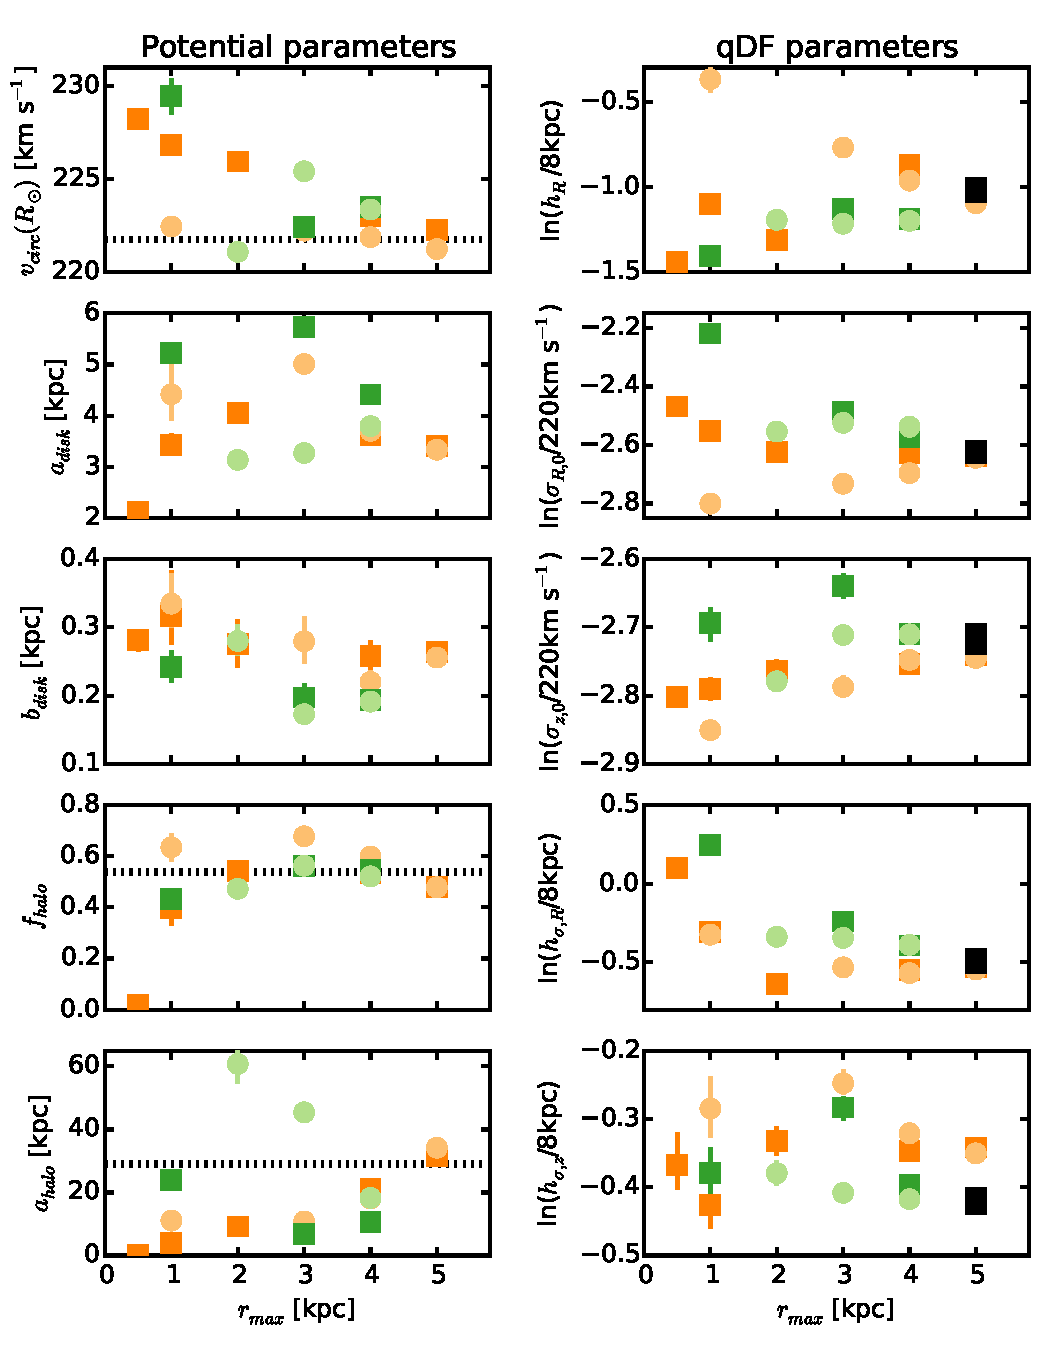
\includegraphics[width=\columnwidth]{fig/MNdHHdiffSph2_violins.pdf}
\caption{Overview over the model parameter estimates (\texttt{MNHH-Pot} parameters on the left, qDF parameters on the right) recovered with \RM{} from data sets drawn from the simulation snapshot at different positions in the galaxy (colour-coded) and of different size ($r_\text{max}$ as indicated on the $x$-axis). The black dotted line shows the known model parameters from the \texttt{expHH-Pot} in Table \Wilma{[TO DO]} (the Miyamoto-Nagai disk parameters $a_\text{disk}$ and $b_\text{disk}$ are related but not directly comparable to an exponential disk scale length and height). The black squares denote the qDF parameters we recovered by fixing the potential to the \texttt{expHH-Pot}, centering a survey volume with $r_\text{kpc}=5$ on the spiral arm at $R=8~\text{kpc}$, and fitting the qDF only. A survey volume with a radial coverage as large as $r_\text{max}=5~\text{kpc}$ is required to properly recover the ''true'' model parameters. \Wilma{[TO DO: Add legend to plot.]} \Wilma{TO DO: Preliminary. Add more results. Make sure that the "true" potential parameters are the final version.} \Wilma{[TO DO: Add additional y-axis on right side of plot with non-log values.]}}
\label{fig:model_parameters}
\end{figure}
%====================

\subsubsection{Size of survey volume}

\Wilma{[To Do: Introductory paragraph.]}

%====================
\begin{figure}[!htbp]
\centering
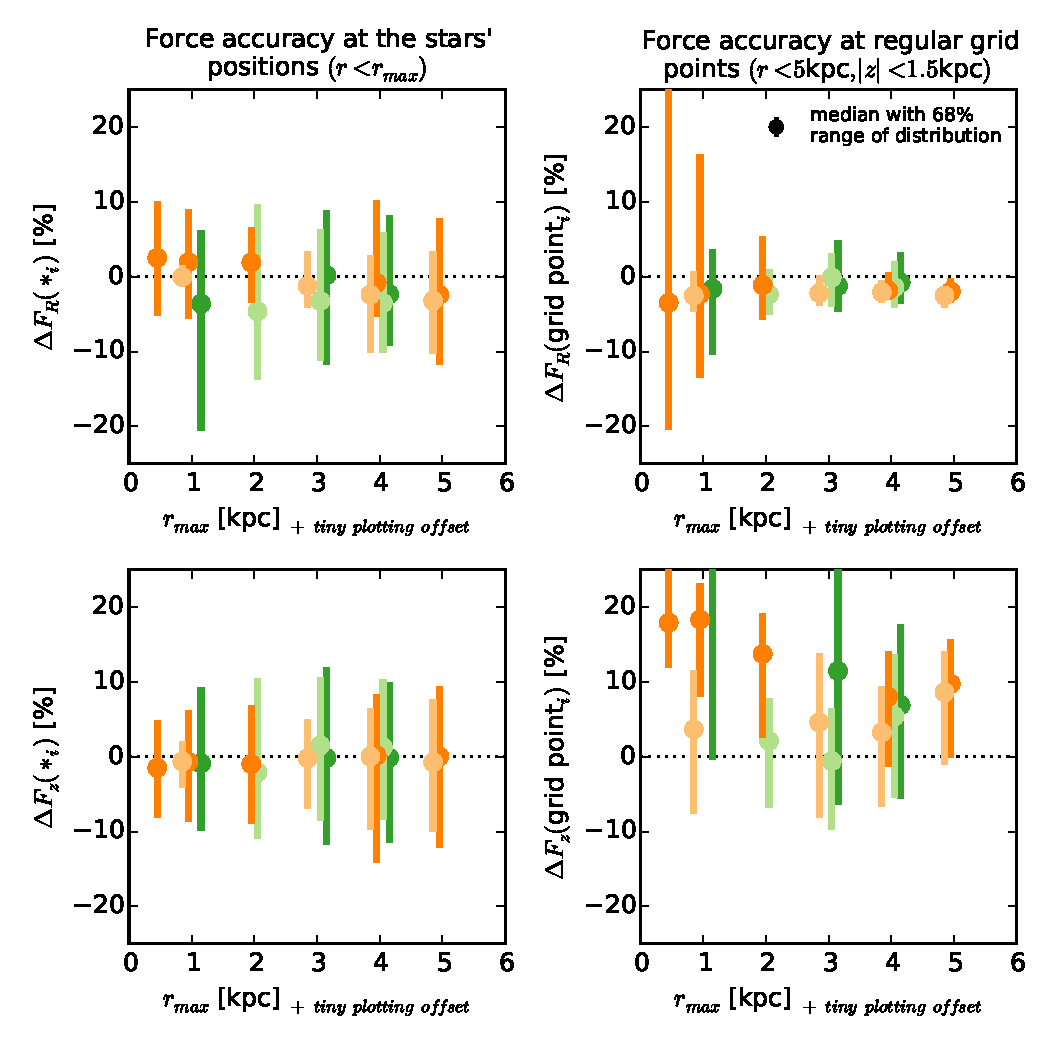
\includegraphics[width=\columnwidth]{fig/MNdHHdiffSph2_bias_in_forces_recovery.pdf}
\caption{\Wilma{TO DO} \Wilma{[TO DO: Make sure all final analyses are in this plot.]}}
\label{fig:forces_bias}
\end{figure}
%====================

\begin{itemize}
\item The first and most important thing to notice is, that we get very close to recovering the true forces at the positions of the stars in the survey volume, no matter how large the survey volume is.
\item The second thing to notice is, that, if we consider not the stars inside the survey volume, but a spatial average of the forces in a large volume ($r_\text{max}=5~\text{kpc}$) independent of the survey volume, the radial forces are overall very well recovered, especially for large survey volumes. There is however a overestimation of $\sim5-20\%$ in the vertical forces (depending on volume size and position) which is induced by the spiral arms (see explanation below).
\item The third thing to notice is that the constraints we get on the spatially averaged forces inside $r<5~\text{kpc}$ is almost as good for the survey volume of $r_\text{max}=3~\text{kpc}$ as compared to survey volumes of $r_\text{max}=4$ or $5~\text{kpc}$. If we had to decide between a $r_\text{max}=3~\text{kpc}$ volume with good data quality and a larger volume with worse data quality, we would loose nothing in terms of force recovery when using the smaller volume. (Only the halo scale length might not be as well constrained, see Figure \ref{fig:model_parameters}).

\item Now let's discuss the reason for the biases that we observe. The peak of the distribution in $\Delta F_R(*_i)$ and $\Delta F_R(g_j)$ is slightly biased towards an underestimation of $|F_{R,M}|$ in our \RM{} models. We think the explanation is the following: Spiral arms are very thin. If a spiral arm crosses the observation volume both its leading side (at large radii) and its trailing side (at small radii) are also in the volume. Stars in the trailing side feel a lower gravitational pull towards the galaxy center than they would if there was no spiral arm. Because there are in general more stars at smaller radii, the \RM{} fit is slightly biased to reproduce in general slightly weaker radial forces. \Wilma{[TO DO: Not 100\% sure but it could be that, when I include the true circular velocity in the vcirc plot above, that one sees that the true vcirc (and therefore FR) is slightly larger than the recovered vcirc.]}

\item The peak of $\Delta F_z(*_i)$ is approximately at 0, while the peak of $\Delta F_z(g_j)$ is strongly biased towards an overestimation of $|F_{z,M}|$. There are much more stars in the spiral arms than in the inter-arm regions, and the stars in the spiral arm feel stronger vertical forces because of the higher disk mass. \RM{} finds a model that in general has much stronger vertical forces than expected for a smooth potential. While the actual vertical forces that the many stars in the spiral arms feel are very well recovered, it becomes obvious when looking at the grid points regularly distributed in space that the \RM{} vertical forces are much stronger. As expected the overestimation is especially strong ($\sim 20 \%$) for small survey volumes dominated by spiral arms, while small volumes dominated by an inter-arm region result in much better estimates for the spatially averaged $F_z(g_j)$ ($\sim5\%$ bias). Large volumes lie somewhere in between (bias of $\sim10\%$).

\item Because the stellar number asymmetry in the trailing vs. leading sides of spiral arms is much smaller than the stellar number asymmetry in spiral arm vs. inter-arm region, the bias is visible in the distribution of $\Delta F_R{*_i}$ ($F_R$ recovery biased only by a few stars $\longrightarrow$ bias for majority of stars visible) and not in $\Delta F_z(*_i)$ (majority of stars biases the fit $\longrightarrow$ we recover $F_z$ for the majority of stars), but becomes really pronounced for $\Delta F_z{g_i}$ (the inter-arm regions dominate when averaging spatially $\longrightarrow$ large overestimation of $F_z$) and stays small for $\Delta F_R{g_i}$ (trailing and leading sides of spiral arms are similarly important when averaging spatially $\longrightarrow$ it becomes visible that the bias is actually not that big).
\end{itemize}

\Wilma{[TO DO: make consistent: $i$ counts stars, $j$ counts grid points.]}


\subsubsection{Influence of spiral arms}

\Wilma{[TO DO: calculate as an alternative statistic the rms deviation in forces and test how plots look with that.]}

%====================
\begin{figure}[!htbp]
\centering
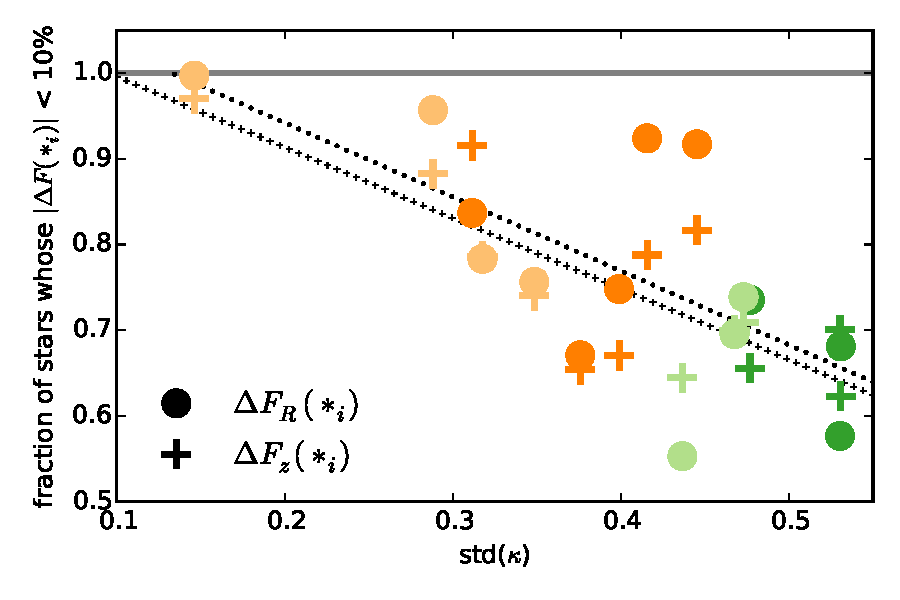
\includegraphics[width=\columnwidth]{fig/MNdHHdiffSph2_plot_stdkappa_vs_frac10star.pdf}
\caption{\Wilma{TO DO} \Wilma{[TO DO: Make sure all final analyses are in this plot.]}}
\label{fig:????}
\end{figure}
%====================

%====================
\begin{figure}[!htbp]
\centering
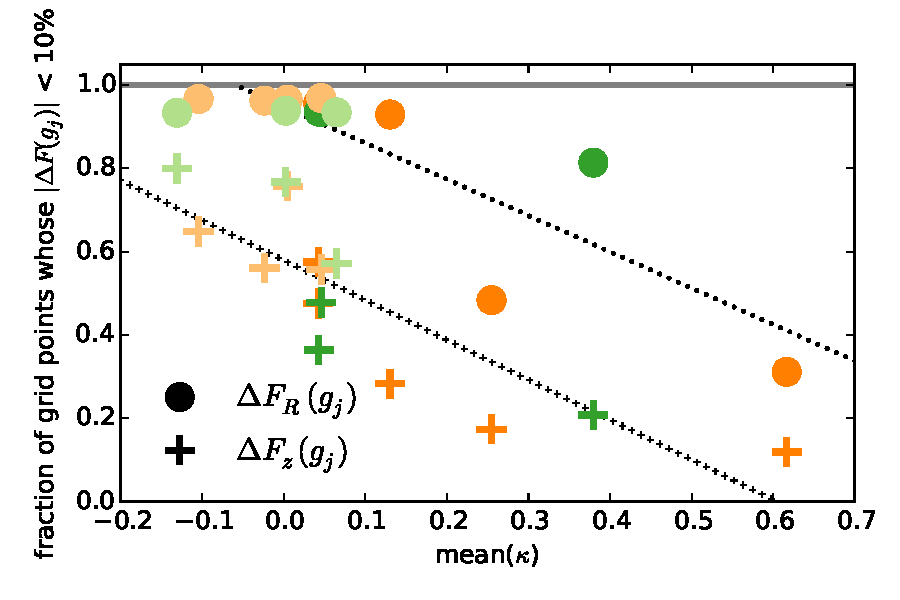
\includegraphics[width=\columnwidth]{fig/MNdHHdiffSph2_plot_meankappa_vs_frac10grid.pdf}
\caption{\Wilma{TO DO} \Wilma{[TO DO: Make sure all final analyses are in this plot.]}}
\label{fig:????}
\end{figure}
%====================

%-----------------------------------------------------------------------------------------------------------------------------------------------------------------------------
%SUMMARY AND CONCLUSION
%-----------------------------------------------------------------------------------------------------------------------------------------------------------------------------
\section{Summary and conclusion}

\bibliography{references_paper2}{}
\bibliographystyle{aasjournal}



\end{document}